\documentclass[11pt,a4paper]{article}

\usepackage[margin=1in]{geometry}
\usepackage{amsmath,amssymb,amsthm}
\usepackage{mathtools}
\usepackage{pgfplots}
\pgfplotsset{compat=1.18}
\usepackage{hyperref}
\usepackage{enumitem}

% Theorem environments
\newtheorem{theorem}{Theorem}[section]
\newtheorem{proposition}[theorem]{Proposition}
\newtheorem{corollary}[theorem]{Corollary}
\newtheorem{definition}[theorem]{Definition}
\newtheorem{example}[theorem]{Example}
\newtheorem{remark}[theorem]{Remark}

\title{\textbf{The Contraction Integral}\\[6pt]
\large An Alternative Geometric Intuition for Integration\\
via Level-Set Contraction}
\author{Nick Navid Yazdani}
\date{March 2026}

\begin{document}
\maketitle

\begin{abstract}
This paper presents an alternative way to think about integration that the author finds
more geometrically intuitive than the standard Riemann-sum construction. The idea is
simple: instead of summing the areas of vertical rectangles, we watch the region under a
curve contract from the bottom up, tracking how much horizontal width is surrendered at
each height. The total area is the accumulated width lost during this contraction. The
underlying identity is classical---it is the layer-cake decomposition of measure theory---and
nothing here replaces or invalidates Riemann sums in any way. This is a matter of personal
geometric taste: the author does not like rectangles. The paper develops the contraction
viewpoint, proves its equivalence to the standard integral, extends it to signed functions and
indefinite integrals, and notes a pleasant computational side effect: an inverse duality that
makes many definite integrals of inverse functions (logarithms, arc-trigonometric functions,
the Lambert~$W$ function) straightforward without integration by parts. These are known
results repackaged through a lens that, for at least one person, makes the whole enterprise
click.
\end{abstract}

\tableofcontents
\newpage

%% ════════════════════════════════════════════════════════════
\section{Introduction: Why This Exists}

I do not like rectangles.

The standard construction of the definite integral proceeds by partitioning the $x$-axis into
subintervals, erecting rectangles, and taking a limit:
\[
\int_a^b f(x)\,dx = \lim_{n\to\infty} \sum_{k=1}^{n} f(x_k^*)\,\Delta x_k.
\]
This is correct.\ It is rigorous.\ It works.\ I have no mathematical objection to it.\ But when
someone asks ``what is the area under this curve?'' and the answer begins with ``first, chop
the $x$-axis into $n$ pieces and build rectangles,'' something about that has always felt like an
unnecessary detour.\ The question is about a curve.\ The answer should, at some level, involve
the curve.

The idea behind this paper is: what if, instead of partitioning the domain and summing
vertical strips, you let the region under the curve shrink?\ At each height~$t$, the curve defines a
horizontal cross-section---the set of $x$-values where the curve is still above~$t$.\ As $t$ rises, that set
gets narrower.\ When it vanishes, the region is gone and you have your area: the total width
surrendered during the contraction.

This is not new mathematics.\ The underlying identity is the \textbf{layer-cake decomposition},
a classical result in measure theory.\ What follows is simply a systematic development of that
identity as a way to think about integration---one that, for me, makes the geometry click in a
way that rectangles never did.

This does not replace Riemann sums.\ Not in generality, not in rigour, not in anything.\
Riemann sums are the foundation.\ This is a lens, not a foundation.\ If you like rectangles, keep
using them.\ If---like me---you find it more natural to watch a region contract than to chop it
into vertical strips, this paper is for you.

What I develop here:
\begin{enumerate}[label=(\roman*)]
\item the contraction viewpoint and its equivalence to the standard integral (via Fubini),
\item an inverse duality that gives a shortcut for many definite integrals of inverse functions,
\item extensions to signed functions (net area) and indefinite integrals (the $+\,C$),
\item worked examples where the contraction viewpoint makes life easier, and
\item a heuristic way to think about why some functions have no elementary antiderivative.
\end{enumerate}

Throughout, I restrict to continuous functions on closed bounded intervals.\ This is a choice
for geometric clarity, not a limitation of the underlying identity.

%% ════════════════════════════════════════════════════════════
\section{Definitions}

\begin{definition}[Level Width Function]\label{def:level-width}
Let $f:[a,b]\to\mathbb{R}_{\geq 0}$ be continuous, and let $\mu$ denote
Lebesgue measure on~$\mathbb{R}$.\ For $t\geq 0$, the \emph{level width} of $f$ at height $t$ is
\[
w_f(t) = \mu\bigl(\{x\in[a,b] : f(x)>t\}\bigr).
\]
\end{definition}

\begin{definition}[Contraction Integral]\label{def:contraction}
Let $f:[a,b]\to\mathbb{R}_{\geq 0}$ be continuous, with $M=\sup_{x\in[a,b]}f(x)$.
The \emph{contraction integral} of $f$ on $[a,b]$ is
\[
\mathcal{C}(f,a,b) = \int_0^M w_f(t)\,dt.
\]
The integrand $w_f(t)$ has a direct geometric reading: it is the horizontal cross-sectional width
of the subgraph of $f$ at height $t$.\ The contraction integral accumulates these widths as $t$ sweeps
from the base to the peak.
\end{definition}

%% ════════════════════════════════════════════════════════════
\section{Properties of the Level Width Function}

\begin{proposition}[Properties of $w_f$]\label{prop:wf}
Let $f:[a,b]\to\mathbb{R}_{\geq 0}$ be continuous with $m=\inf f$ and $M=\sup f$.\ Then:
\begin{enumerate}[label=(\roman*)]
\item $w_f$ is non-increasing on $[0,\infty)$.
\item $w_f(t) = b-a$ for all $t<m$.
\item $w_f(t) = 0$ for all $t\geq M$.
\item $w_f$ is right-continuous on $[0,\infty)$.
\item If $f$ is strictly monotone on a subinterval $I$, then $w_f$ is strictly decreasing on $f(I)$.
\end{enumerate}
\end{proposition}

\begin{proof}
(i) If $s<t$, then $\{f>t\}\subseteq\{f>s\}$, so $w_f(t)\leq w_f(s)$.

(ii) If $t<m$, then $f(x)>t$ for all $x\in[a,b]$, so $\{f>t\}=[a,b]$.

(iii) If $t\geq M$, then $f(x)\leq M\leq t$ for all $x$, so $\{f>t\}=\varnothing$.

(iv) Fix $t\geq 0$.\ For each $n\geq 1$, define $E_n=\{x\in[a,b]:f(x)>t+1/n\}$.\ Then $E_1\subseteq E_2\subseteq\cdots$ and
\[
\bigcup_{n=1}^{\infty}E_n = \{x\in[a,b]:f(x)>t\}.
\]
By continuity of measure from below, $\mu(E_n)\to\mu(\{f>t\})$, i.e., $w_f(t+1/n)\to w_f(t)$.\ Since $w_f$ is non-increasing, this establishes right-continuity at~$t$.

(v) If $f$ is strictly increasing on $I=[\alpha,\beta]$, then for $f(\alpha)\leq s<t\leq f(\beta)$, the set $\{x\in I:f(x)>t\}$ is strictly contained in $\{x\in I:f(x)>s\}$, and both are intervals of positive measure.\ The contribution from~$I$ to~$w_f$ is therefore strictly decreasing on $[f(\alpha),f(\beta)]$.
\end{proof}

\begin{remark}\label{rem:measurable}
The level width function and the contraction integral are well defined for any non-negative measurable function~$f$; continuity is not required.\ The equivalence theorem (Section~\ref{sec:equiv}) likewise holds in the measurable setting, where it is the standard layer-cake formula.\ We restrict to continuous functions throughout for geometric concreteness.
\end{remark}

%% ════════════════════════════════════════════════════════════
\section{Equivalence Theorem}\label{sec:equiv}

\begin{theorem}[Equivalence of Contraction and Riemann Integrals]\label{thm:equiv}
Let $f:[a,b]\to\mathbb{R}_{\geq 0}$ be continuous.\ Then
\[
\mathcal{C}(f,a,b) = \int_a^b f(x)\,dx.
\]
\end{theorem}

\begin{proof}
The subgraph of $f$ is the set
\[
G_f = \{(x,t)\in\mathbb{R}^2 : a\leq x\leq b,\; 0\leq t\leq f(x)\}.
\]
Its area is computed by the Lebesgue integral $\int_a^b f(x)\,dx$.\ We apply Fubini--Tonelli to the indicator function $\mathbf{1}_{G_f}(x,t)$:
\begin{align*}
\int_a^b f(x)\,dx
&= \int_a^b\!\left(\int_0^{f(x)}dt\right)dx
= \int_a^b\int_0^M \mathbf{1}_{\{f(x)>t\}}\,dt\,dx \\
&= \int_0^M\!\left(\int_a^b \mathbf{1}_{\{f(x)>t\}}\,dx\right)dt
= \int_0^M w_f(t)\,dt
= \mathcal{C}(f,a,b).
\end{align*}
The exchange of integration order is justified by Tonelli's theorem, since the integrand is non-negative and measurable.
\end{proof}

\begin{remark}\label{rem:layer-cake}
This identity is the layer-cake decomposition, well known in measure theory and functional analysis (see, e.g., Lieb and Loss, \emph{Analysis}, Chapter~1).\ I am not claiming to have discovered it.\ I am claiming it is a better way to think about area than rectangles, at least for the way my brain works.
\end{remark}

%% ════════════════════════════════════════════════════════════
\section{The Contraction Process}

The contraction integral admits a natural interpretation as a process: the region under $f$ is consumed from the bottom up by a continuously rising horizontal line.

\begin{definition}[Accumulated Area]\label{def:accum}
For $s\in[0,M]$, define the accumulated area at contraction height~$s$:
\[
A_f(s) = \int_0^s w_f(t)\,dt.
\]
\end{definition}

\begin{proposition}[Properties of the Contraction Process]\label{prop:process}
The function $A_f$ satisfies:
\begin{enumerate}[label=(\roman*)]
\item $A_f(0) = 0$.
\item $A_f(M) = \mathcal{C}(f,a,b) = \int_a^b f(x)\,dx$.
\item $A_f$ is continuous and non-decreasing on $[0,M]$.
\item $A_f$ is concave on $[0,M]$.
\item $A_f'(s) = w_f(s)$ at every point of continuity of $w_f$.
\end{enumerate}
\end{proposition}

\begin{proof}
Properties (i)--(iii) and (v) follow directly from the definition and the fundamental theorem of calculus for Lebesgue integrals.\ For (iv): since $w_f$ is non-increasing (Proposition~\ref{prop:wf}(i)), its integral $A_f$ is concave.
\end{proof}

The concavity of $A_f$ means the contraction consumes area fastest near the base (where the region is widest) and slowest near the peak.\ Note that this is a statement about the accumulated area, not about $w_f$ itself; $w_f$ may be either convex or concave depending on the shape of~$f$ (see Section~\ref{sec:convexity}).

\begin{center}
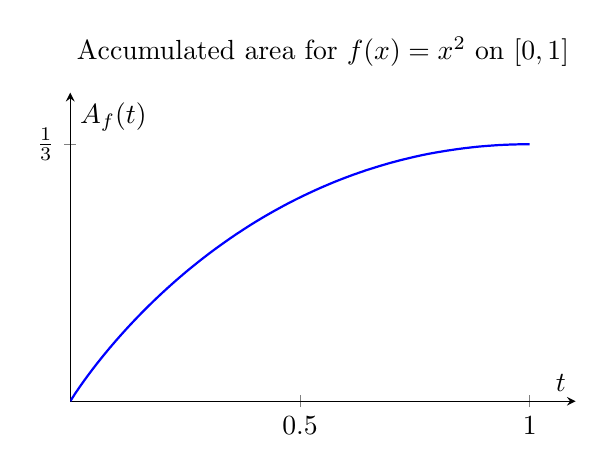
\begin{tikzpicture}
\begin{axis}[
    width=8cm, height=5.5cm,
    xlabel={$t$}, ylabel={$A_f(t)$},
    xmin=0, xmax=1.1, ymin=0, ymax=0.4,
    axis lines=middle,
    ytick={0.333},
    yticklabels={$\frac{1}{3}$},
    xtick={0.5,1},
    title={Accumulated area for $f(x)=x^2$ on $[0,1]$},
    samples=100,
    domain=0:1,
]
\addplot[thick, blue] {x - (2/3)*x^(3/2)};
\end{axis}
\end{tikzpicture}
\end{center}

%% ════════════════════════════════════════════════════════════
\section{Inverse Duality}

The most useful thing that falls out of the contraction viewpoint is a duality between a function and its inverse.

\begin{theorem}[Inverse Duality --- General Form]\label{thm:duality}
Let $f:[a,b]\to\mathbb{R}$ be continuous and strictly increasing.\ Then
\[
\int_a^b f(x)\,dx + \int_{f(a)}^{f(b)} f^{-1}(y)\,dy = b\,f(b) - a\,f(a).
\]
\end{theorem}

\begin{proof}
By integration by parts (or equivalently, substitution with $y=f(x)$):
\[
\int_a^b f(x)\,dx = \bigl[x\,f(x)\bigr]_a^b - \int_a^b x\,f'(x)\,dx
= b\,f(b) - a\,f(a) - \int_{f(a)}^{f(b)} f^{-1}(y)\,dy,
\]
where the last step substitutes $y=f(x)$, $dy=f'(x)\,dx$, and $x=f^{-1}(y)$.
\end{proof}

\begin{corollary}[Normalized Inverse Duality]\label{cor:norm-duality}
If additionally $f(a)=0$ and we write $M=f(b)$, then
\[
\int_a^b f(x)\,dx = bM - \int_0^M f^{-1}(t)\,dt.
\]
The curve $y=f(x)$ partitions the rectangle $[0,b]\times[0,M]$ into two complementary regions: the area under $f$ and the area under $f^{-1}$.\ Their sum is $bM$.
\end{corollary}

\begin{center}
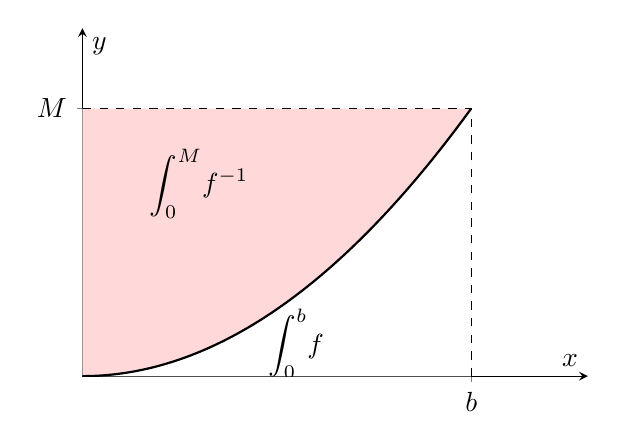
\begin{tikzpicture}
\begin{axis}[
    width=8cm, height=6cm,
    xlabel={$x$}, ylabel={$y$},
    xmin=0, xmax=1.3, ymin=0, ymax=1.3,
    axis lines=middle,
    xtick={1}, xticklabels={$b$},
    ytick={1}, yticklabels={$M$},
    samples=100,
    domain=0:1,
]
% Area under f
\addplot[thick, blue, fill=blue!15, draw=none, domain=0:1] {x^2} \closedcycle;
% Area under f^{-1} (i.e. above f, in the rectangle)
\addplot[thick, red, fill=red!15, draw=none, domain=0:1] {1} \closedcycle;
\addplot[thick, red, fill=white, draw=none, domain=0:1] {x^2} \closedcycle;
% The curve
\addplot[thick, black, domain=0:1] {x^2};
% Rectangle outline
\draw[dashed] (axis cs:1,0) -- (axis cs:1,1) -- (axis cs:0,1);
% Labels
\node at (axis cs:0.55,0.12) {$\displaystyle\int_0^b\! f$};
\node at (axis cs:0.3,0.72) {$\displaystyle\int_0^M\! f^{-1}$};
\end{axis}
\end{tikzpicture}

\smallskip
Duality: $\int\! f + \int\! f^{-1} = bM$ (when $f(a)=0$)
\end{center}

\begin{remark}\label{rem:non-injective-duality}
The inverse duality generalises to non-injective functions via the level width function.\ For arbitrary continuous $f\geq 0$, the identity $\mathcal{C}(f,a,b)=\int_0^M w_f(t)\,dt$ still holds, with $w_f(t)$ being the total measure of the super-level set.\ It simply cannot be expressed in terms of a single inverse function.
\end{remark}

%% ════════════════════════════════════════════════════════════
\section{Extension to Signed Functions}

The contraction integral as defined in Section~\ref{def:contraction} applies to non-negative functions.\ To handle functions that cross the $x$-axis---and thereby recover the signed (``net'') area required in physics, engineering, and the general Fundamental Theorem of Calculus---we decompose $f$ into its positive and negative parts.

\begin{definition}[Positive and Negative Parts]\label{def:pos-neg}
For $f:[a,b]\to\mathbb{R}$ continuous, define:
\[
f^+(x) = \max(f(x),0), \qquad f^-(x) = \max(-f(x),0).
\]
Then $f = f^+ - f^-$ and $|f| = f^+ + f^-$, with $f^+,f^-\geq 0$.
\end{definition}

\begin{definition}[Signed Contraction Integral]\label{def:signed}
For $f:[a,b]\to\mathbb{R}$ continuous, define
\[
\mathcal{C}^{\pm}(f,a,b) = \mathcal{C}(f^+,a,b) - \mathcal{C}(f^-,a,b)
\]
where each term is the (non-negative) contraction integral of the respective part.
\end{definition}

Geometrically: the region above the $x$-axis contracts upward from height~$0$ to $\sup f^+$, accumulating positive area.\ The region below the $x$-axis contracts downward from height~$0$ to $-\inf f$ (or equivalently, $f^-$ contracts upward from~$0$ to $\sup f^- = -\inf f$), accumulating area that enters with a negative sign.\ The net integral is the difference.

\begin{theorem}\label{thm:signed}
For $f:[a,b]\to\mathbb{R}$ continuous,
\[
\mathcal{C}^{\pm}(f,a,b) = \int_a^b f(x)\,dx.
\]
\end{theorem}

\begin{proof}
By Theorem~\ref{thm:equiv} applied to $f^+$ and $f^-$ separately:
\[
\mathcal{C}^{\pm}(f,a,b) = \int_a^b f^+(x)\,dx - \int_a^b f^-(x)\,dx = \int_a^b (f^+-f^-)(x)\,dx = \int_a^b f(x)\,dx. \qedhere
\]
\end{proof}

\begin{remark}\label{rem:signed-level}
Equivalently, the signed contraction can be expressed as a single integral over the full range of~$f$.\ Define the signed level width:
\[
w_f^{\pm}(t) = \begin{cases}
+\mu(\{x\in[a,b]:f(x)>t\}) & \text{if } t\geq 0,\\
-\mu(\{x\in[a,b]:f(x)<t\}) & \text{if } t<0.
\end{cases}
\]
Then
\[
\int_a^b f(x)\,dx = \int_{\inf f}^{\sup f} w_f^{\pm}(t)\,dt.
\]
The contraction now sweeps the entire range of~$f$, from its minimum to its maximum: below the $x$-axis it contracts sub-level sets (accumulating negative area), and above it contracts super-level sets (accumulating positive area).
\end{remark}

\begin{example}[$f(x)=\sin(x)$ on $[0,2\pi]$]\label{ex:sin-signed}
Here $f^+(x)=\sin(x)$ on $[0,\pi]$ (and zero elsewhere), $f^-(x)=-\sin(x)$ on $[\pi,2\pi]$ (and zero elsewhere).\ By symmetry, $\mathcal{C}(f^+,0,2\pi)=2$ and $\mathcal{C}(f^-,0,2\pi)=2$, so $\mathcal{C}^{\pm}(\sin,0,2\pi) = 2-2=0$, as expected.
\end{example}

%% ════════════════════════════════════════════════════════════
\section{Extension to Indefinite Integrals}

The contraction framework extends naturally to indefinite integrals by allowing the domain boundary to move.

\begin{definition}[Contraction Antiderivative]\label{def:antideriv}
Let $f:[a,b]\to\mathbb{R}_{\geq 0}$ be continuous.\ For $x\in[a,b]$, define the level width restricted to $[a,x]$:
\[
w_{f,x}(t) = \mu\bigl(\{s\in[a,x]:f(s)>t\}\bigr)
\]
and the contraction antiderivative:
\[
F(x) = \int_0^{M(x)} w_{f,x}(t)\,dt
\]
where $M(x)=\sup_{s\in[a,x]}f(s)$.
\end{definition}

As $x$ increases by an infinitesimal amount~$dx$, the level set $\{s\in[a,x]:f(s)>t\}$ grows by~$dx$ at every height $t\in[0,f(x))$, and does not grow for $t\geq f(x)$.\ The infinitesimal area contributed is therefore:
\[
dF = \left(\int_0^{f(x)}dt\right)dx = f(x)\,dx.
\]

\begin{theorem}[Contraction FTC]\label{thm:contraction-ftc}
Let $f:[a,b]\to\mathbb{R}_{\geq 0}$ be continuous.\ The contraction antiderivative $F$ satisfies:
\begin{enumerate}[label=(\roman*)]
\item $F(a) = 0$.
\item $F'(x) = f(x)$ for all $x\in[a,b]$.
\item $F(b) = \mathcal{C}(f,a,b) = \int_a^b f(x)\,dx$.
\end{enumerate}
\end{theorem}

\begin{proof}
(i) At $x=a$, the domain $[a,a]$ is a single point, so $w_{f,a}(t)=0$ for all~$t$, giving $F(a)=0$.

(ii) By Theorem~\ref{thm:equiv} applied to the restriction of $f$ to $[a,x]$:
\[
F(x) = \int_0^{M(x)}w_{f,x}(t)\,dt = \int_a^x f(s)\,ds.
\]
By the standard Fundamental Theorem of Calculus, $F'(x)=f(x)$.

(iii) $F(b)=\int_a^b f(s)\,ds = \mathcal{C}(f,a,b)$.
\end{proof}

\begin{remark}[The constant of integration]\label{rem:constant}
The $+\,C$ of classical indefinite integration corresponds to the choice of the base point~$a$.\ Two contraction antiderivatives $F_1$ (based at~$a_1$) and $F_2$ (based at~$a_2$) satisfy
\[
F_1(x) - F_2(x) = \int_{a_2}^{a_1} f(s)\,ds = \text{constant},
\]
which is independent of~$x$.\ The ``arbitrary constant'' is thus the net area between the two base points---it has a direct geometric meaning within the contraction framework, rather than being an algebraic artefact.

The geometric picture of the indefinite integral: as $x$ sweeps rightward from~$a$, the contraction ``window'' $[a,x]$ widens.\ At each position~$x$, the level-set structure of $f$ on $[a,x]$ determines a complete contraction process.\ The value $F(x)$ is the terminal value of that contraction.\ The derivative $F'(x)=f(x)$ says: the rate at which area accumulates as the window widens equals the height of the curve at the window's right edge.

For signed functions, the extension follows immediately from Section~7: define $F(x)=\mathcal{C}^{\pm}(f,a,x)$.
\end{remark}

%% ════════════════════════════════════════════════════════════
\section{Computational Consequences}

The inverse duality has a pleasant computational side effect: it provides a uniform method for evaluating definite integrals of inverse functions without the usual integration-by-parts dance.

\begin{corollary}\label{cor:comp}
Let $f:[a,b]\to[0,M]$ be continuous and strictly increasing with $f(a)=0$, and suppose $g=f^{-1}$ has an explicitly computable antiderivative on $[0,M]$.\ Then the definite integral of $f$ can be evaluated by the duality formula:
\[
\int_a^b f(x)\,dx = bM - \int_0^M g(t)\,dt.
\]
\end{corollary}

In cases where the forward function $g=f^{-1}$ is simpler to integrate than $f$ itself, this bypasses the usual integration-by-parts workflow.\ The method relocates the problem to the forward function, which is often more elementary.

\subsection{Worked Examples}

\begin{example}[$\int_0^1\arcsin(x)\,dx$]\label{ex:arcsin}
The standard approach requires integration by parts with $u=\arcsin(x)$, $dv=dx$, followed by a substitution involving $\frac{x}{\sqrt{1-x^2}}$.

\emph{Via duality.}\ Here $f(x)=\arcsin(x)$, so $f^{-1}(t)=\sin(t)$, $b=1$, and $M=\pi/2$:
\[
\int_0^1\arcsin(x)\,dx = 1\cdot\frac{\pi}{2} - \int_0^{\pi/2}\sin(t)\,dt = \frac{\pi}{2} - \bigl[-\cos(t)\bigr]_0^{\pi/2} = \frac{\pi}{2}-1.
\]
\end{example}

\begin{example}[$\int_1^e\ln(x)\,dx$]\label{ex:ln}
The standard approach requires integration by parts.

\emph{Via duality.}\ Here $f(x)=\ln(x)$ on $[1,e]$, so $f^{-1}(t)=e^t$, $f(1)=0$, $b=e$, and $M=1$:
\[
\int_1^e\ln(x)\,dx = e\cdot 1 - \int_0^1 e^t\,dt = e-(e-1) = 1.
\]
\end{example}

\begin{example}[$\int_0^1\arctan(x)\,dx$]\label{ex:arctan}
The standard approach requires integration by parts.

\emph{Via duality.}\ Here $f^{-1}(t)=\tan(t)$, $b=1$, $M=\pi/4$:
\[
\int_0^1\arctan(x)\,dx = \frac{\pi}{4} - \int_0^{\pi/4}\tan(t)\,dt = \frac{\pi}{4} - \bigl[-\ln\cos(t)\bigr]_0^{\pi/4} = \frac{\pi}{4} - \frac{\ln 2}{2}.
\]
\end{example}

\begin{example}[The Lambert $W$ function: $\int_0^e W(x)\,dx$]\label{ex:lambert}
The Lambert $W$ function satisfies $W(x)e^{W(x)}=x$.\ Evaluating its definite integral by standard methods requires special-function theory.

\emph{Via duality.}\ The inverse of $W$ is $g(t)=te^t$, and $W(e)=1$, so $M=1$:
\[
\int_0^e W(x)\,dx = e\cdot 1 - \int_0^1 te^t\,dt = e - \bigl[te^t - e^t\bigr]_0^1 = e-1.
\]
The duality has relocated the problem from a special function to an elementary one.
\end{example}

\begin{example}[$\int_0^1\operatorname{arcsinh}(x)\,dx$]\label{ex:arcsinh}
The standard approach requires integration by parts with $\sqrt{1+x^2}$.

\emph{Via duality.}\ Here $f^{-1}(t)=\sinh(t)$, and $M=\operatorname{arcsinh}(1)=\ln(1+\sqrt{2})$:
\[
\int_0^1\operatorname{arcsinh}(x)\,dx = \ln(1+\sqrt{2}) - \int_0^{\ln(1+\sqrt{2})}\sinh(t)\,dt = \ln(1+\sqrt{2}) - (\sqrt{2}-1).
\]
\end{example}

\subsection{Summary of Computational Gains}

\begin{center}
\begin{tabular}{l l l}
\textbf{Function $f$} & \textbf{Standard method} & \textbf{Dual computation (integrate $f^{-1}$)} \\
\hline
$\ln(x)$              & IBP                       & $\int e^t\,dt$ \\
$\arcsin(x)$          & IBP + substitution         & $\int\sin(t)\,dt$ \\
$\arctan(x)$          & IBP                       & $\int\tan(t)\,dt$ \\
$\arccos(x)$          & IBP + substitution         & $\int\cos(t)\,dt$ \\
$\operatorname{arcsinh}(x)$ & IBP + $\sqrt{1+x^2}$ & $\int\sinh(t)\,dt$ \\
$\operatorname{arctanh}(x)$ & IBP + partial fractions & $\int\tanh(t)\,dt$ \\
$W(x)$ (Lambert)      & Special function theory    & $\int te^t\,dt$ \\
\end{tabular}
\end{center}

%% ════════════════════════════════════════════════════════════
\section{The Non-Injective Case}

When $f$ is not injective, the super-level set $\{x\in[a,b]:f(x)>t\}$ may consist of multiple disjoint intervals.\ The contraction integral applies without modification: $w_f(t)$ is the total measure of the super-level set.

\begin{example}[$f(x)=\sin(x)$ on $[0,\pi]$]\label{ex:sin-non-inj}
At height $t\in(0,1)$, the equation $\sin(x)=t$ has two solutions in $[0,\pi]$: $x_1=\arcsin(t)$ and $x_2=\pi-\arcsin(t)$.\ The super-level set is the single interval $(\arcsin(t),\pi-\arcsin(t))$, so
\[
w_f(t) = \pi - 2\arcsin(t).
\]
Therefore
\[
\mathcal{C}(\sin,0,\pi) = \int_0^1\bigl(\pi-2\arcsin(t)\bigr)\,dt = \pi - 2\!\left(\frac{\pi}{2}-1\right) = 2.
\]
\end{example}

\begin{remark}[Highly oscillatory functions]\label{rem:oscillatory}
For functions that oscillate frequently---such as $\sin(1/x)$ near the origin---the super-level set at each height~$t$ may consist of infinitely many disjoint intervals.\ The contraction integral remains well defined (the total measure is finite), but computing $w_f(t)$ may be more involved than a standard vertical approach.\ The contraction viewpoint is most computationally advantageous when the level-set structure is simple; for highly oscillatory functions, the standard approach may be preferable.
\end{remark}

%% ════════════════════════════════════════════════════════════
\section{Connection to the Fundamental Theorem of Calculus}

In the contraction framework, the Fundamental Theorem of Calculus takes a transparent form.\ If $F'(x)=f(x)$ with $F(a)=0$, then
\[
\int_a^b f(x)\,dx = F(b).
\]
The contraction view: $F(b)$ is the terminal value of the contraction process.\ The standard FTC parametrises accumulated area by~$x$ (sweeping left to right); the contraction parametrises it by~$t$ (sweeping bottom to top).\ Both are monotone reparametrisations of the same underlying quantity.

With the indefinite integral extension of Section~8, the connection is even tighter: the contraction antiderivative $F(x)=\int_0^{M(x)}w_{f,x}(t)\,dt$ satisfies $F'=f$ and $F(a)=0$.\ It is the unique antiderivative vanishing at~$a$, constructed entirely from horizontal geometry.

%% ════════════════════════════════════════════════════════════
\section{Convexity and the Level Width Function}\label{sec:convexity}

The contraction exposes a relationship between the convexity of $f$ and the shape of its level width function.

\begin{proposition}\label{prop:convexity}
Let $f:[a,b]\to\mathbb{R}_{\geq 0}$ be $C^2$ and strictly increasing with $f(a)=0$ and $f'>0$ on $[a,b]$.
\begin{enumerate}[label=(\roman*)]
\item If $f$ is convex ($f''>0$), then $w_f$ is convex on $[0,M]$.
\item If $f$ is concave ($f''<0$), then $w_f$ is concave on $[0,M]$.
\end{enumerate}
\end{proposition}

\begin{proof}
Since $f$ is strictly increasing with $f(a)=0$, we have $w_f(t)=b-f^{-1}(t)$ for $t\in[0,M]$.\ Differentiating twice:
\[
w_f'(t) = \frac{-1}{f'(f^{-1}(t))}, \qquad
w_f''(t) = \frac{f''(f^{-1}(t))}{\bigl(f'(f^{-1}(t))\bigr)^3}.
\]
Since $f'>0$, the denominator is strictly positive.\ Therefore $\operatorname{sgn}(w_f'') = \operatorname{sgn}(f'')$.
\end{proof}

\begin{remark}\label{rem:no-contradict}
This does not contradict the concavity of the accumulated area $A_f$ established in Proposition~\ref{prop:process}(iv).\ The function $A_f$ is concave because its derivative $A_f'=w_f$ is non-increasing.\ A function can be simultaneously non-increasing and convex: for example, $w_f(t)=1-\sqrt{t}$ on $[0,1]$ is non-increasing (derivative $<0$) and convex (second derivative $>0$).\ The concavity of $A_f$ and the convexity of $w_f$ are compatible properties at different levels of the hierarchy.
\end{remark}

%% ════════════════════════════════════════════════════════════
\section{A Way to Think About Intractability}

One thing I find satisfying about the contraction viewpoint: it gives you a way to think about why some functions resist closed-form integration, rather than just accepting ``Liouville says no.''

The contraction provides two independent routes to the area: integrate $f$ along $x$, or integrate $w_f$ (equivalently, $f^{-1}$ in the injective case) along $t$.\ This suggests a rough classification.

\begin{definition}[Tractability Classes --- Heuristic]\label{def:tractability}
Let $f:[a,b]\to\mathbb{R}_{\geq 0}$ be continuous.\ We say informally that:
\begin{enumerate}[label=(\roman*)]
\item $f$ is \emph{bilaterally tractable} if both $\int f(x)\,dx$ and $\int w_f(t)\,dt$ can be evaluated in elementary closed form.
\item $f$ is \emph{unilaterally tractable} if exactly one of the two can be so evaluated.
\item $f$ is \emph{bilaterally intractable} if neither can be so evaluated.
\end{enumerate}
\end{definition}

\begin{example}[Representatives of each class]\label{ex:tract-class}
\leavevmode
\begin{itemize}
\item \emph{Bilaterally tractable:} $x^n$, $\sin(x)$, $e^x$, polynomials.
\item \emph{Unilaterally tractable:} $\arcsin(x)$, $\ln(x)$, $\arctan(x)$, $W(x)$.
\item \emph{Bilaterally intractable:} $e^{x^2}$ (inverse: $\sqrt{\ln t}$; neither has an elementary antiderivative).
\end{itemize}
\end{example}

\begin{remark}\label{rem:heuristic}
This taxonomy is heuristic.\ The formal question of whether a given function possesses an elementary antiderivative belongs to differential algebra (Liouville's theorem and its extensions).\ The contraction viewpoint does not settle such questions; it provides a second vantage point from which to attempt evaluation.\ When both orientations resist elementary evaluation, this is suggestive of intrinsic complexity, but the formal proof of non-elementarity still requires the methods of differential algebra.
\end{remark}

%% ════════════════════════════════════════════════════════════
\section{Where This Doesn't Help}

The contraction viewpoint is not universally better than rectangles---it is differently shaped, and that shape fits some problems and not others.\ Here are the cases where it does not help, or actively makes things harder.

\medskip
\noindent\textbf{Restriction to continuous functions.}\quad
The present paper works exclusively with continuous functions on closed bounded intervals.\ The underlying layer-cake identity holds for all non-negative measurable functions (Remark~\ref{rem:measurable}), but the geometric language of ``contracting level sets'' is most natural when the super-level sets are open intervals with well-behaved boundaries.\ For highly discontinuous functions (e.g., the Dirichlet function), computing $w_f(t)$ becomes a measure-theoretic exercise rather than a geometric one.\ The contraction viewpoint is designed for functions where the level-set structure is geometrically transparent.

\medskip
\noindent\textbf{Highly oscillatory functions.}\quad
When $f$ oscillates rapidly---such as $\sin(1/x)$ near the origin---the super-level set at each height~$t$ may consist of infinitely many disjoint intervals.\ The total measure $w_f(t)$ remains well defined, but its explicit computation may be more involved than a standard vertical integral.\ The contraction viewpoint is most advantageous when the level-set structure is simple; for highly oscillatory functions, the standard partition approach may be the more practical route.

\medskip
\noindent\textbf{Higher dimensions.}\quad
The layer-cake formula generalises to higher dimensions: for $f:\mathbb{R}^n\to\mathbb{R}_{\geq 0}$ measurable,
\[
\int_{\mathbb{R}^n}f(x)\,dx = \int_0^{\infty}\mu_n(\{x:f(x)>t\})\,dt,
\]
where $\mu_n$ is $n$-dimensional Lebesgue measure.\ This connects the contraction viewpoint to Cavalieri's principle.\ However, the inverse duality---which gives the 1D version much of its computational power---does not generalise directly, since a multi-variable function typically has no single-valued inverse.\ The higher-dimensional contraction remains valid as a formula but loses the shortcut that makes the 1D case so effective.

\medskip
\noindent\textbf{Measure-zero features.}\quad
The contraction integral, like any Lebesgue-based integral, is insensitive to modifications on sets of measure zero.\ A function with isolated spikes (e.g., a point mass) produces identical contraction profiles to the function without the spikes.\ This is a property of area itself, not of the contraction method specifically---the Riemann integral shares this insensitivity for integrable functions---but it is worth noting that the contraction's geometric language of ``width surrendered'' naturally excludes features with zero width.

%% ════════════════════════════════════════════════════════════
\section{Illustrative Symbolic Verification}

As a sanity check (not as evidence---the proof already handles that), I verified every theorem and worked example in this paper against the standard Riemann integral in SymPy.\ The verification script checks each result two ways where applicable: by direct symbolic integration and by the duality formula.

\medskip
\noindent\textbf{Theorems verified:}

\begin{center}
\begin{tabular}{l l l}
\textbf{Result} & \textbf{Test} & \textbf{Status} \\
\hline
Theorem~\ref{thm:equiv} & $\int_0^1(1-\sqrt{t})\,dt = \int_0^1 x^2\,dx = \tfrac{1}{3}$ & $\checkmark$ \\[3pt]
Theorem~\ref{thm:duality} & $\int_0^1 x\,dx + \int_0^1 t\,dt = 1\cdot 1$ & $\checkmark$ \\[3pt]
Theorem~\ref{thm:signed} & $\mathcal{C}^{\pm}(\sin,0,2\pi)=0$ & $\checkmark$ \\[3pt]
Theorem~\ref{thm:contraction-ftc} & $F(x)=\tfrac{x^3}{3}$, \; $F'(x)=x^2$, \; $F(0)=0$ & $\checkmark$ \\
\end{tabular}
\end{center}

\medskip
\noindent\textbf{Worked examples verified (direct and dual routes):}

\begin{center}
\begin{tabular}{l l l l}
\textbf{Example} & \textbf{Function} & \textbf{Paper's value} & \textbf{Status} \\
\hline
\ref{ex:arcsin} & $\arcsin(x)$ on $[0,1]$ & $\pi/2-1$ & $\checkmark$ \\[2pt]
\ref{ex:ln} & $\ln(x)$ on $[1,e]$ & $1$ & $\checkmark$ \\[2pt]
\ref{ex:arctan} & $\arctan(x)$ on $[0,1]$ & $\pi/4 - \tfrac{\ln 2}{2}$ & $\checkmark$ \\[2pt]
\ref{ex:lambert} & $W(x)$ on $[0,e]$ & $e-1$ & $\checkmark$ \\[2pt]
\ref{ex:arcsinh} & $\operatorname{arcsinh}(x)$ on $[0,1]$ & $\ln(1{+}\sqrt{2})-(\sqrt{2}{-}1)$ & $\checkmark^{\dagger}$ \\[2pt]
\ref{ex:sin-non-inj} & $\sin(x)$ on $[0,\pi]$ & $2$ & $\checkmark$ \\
\end{tabular}
\end{center}

\noindent${}^{\dagger}$\,The dual route for Example~\ref{ex:arcsinh} produces $\ln(1{+}\sqrt{2}) - \cosh(\ln(1{+}\sqrt{2})) + 1$; SymPy does not symbolically reduce $\cosh(\ln(1{+}\sqrt{2}))$ to $\sqrt{2}$, but numerical evaluation confirms agreement to machine precision ($<10^{-15}$).

\medskip
\noindent\textbf{Sanity-check table} (contraction vs.\ Riemann, as before):

\begin{center}
\begin{tabular}{l c c c}
\textbf{Function} & \textbf{Domain} & \textbf{Riemann} & \textbf{Contraction} \\
\hline
$x^2$       & $[0,1]$   & $1/3$ & $1/3$ \\
$\sin(x)$   & $[0,\pi]$ & $2$   & $2$   \\
$x^3$       & $[0,1]$   & $1/4$ & $1/4$ \\
$\sqrt{x}$  & $[0,1]$   & $2/3$ & $2/3$ \\
$x$         & $[0,1]$   & $1/2$ & $1/2$ \\
$x^4$       & $[0,1]$   & $1/5$ & $1/5$ \\
$2x^2+x$    & $[0,1]$   & $7/6$ & $7/6$ \\
\end{tabular}
\end{center}

\noindent The full verification script (22 checks, all passing) is available as supplementary material.\footnote{\texttt{verify\_contraction\_final.py}, included with this paper.\ Requires SymPy $\geq$~1.12.}

%% ════════════════════════════════════════════════════════════
\section{Conclusion}

None of this is revolutionary.\ The layer-cake decomposition has been in the measure theory textbooks for decades.\ The inverse duality is a repackaging of a standard integration-by-parts identity.\ The signed and indefinite extensions are straightforward constructions on top of existing machinery.

What this paper is, honestly, is one person's attempt to build an intuition for integration that doesn't start with rectangles.\ The contraction viewpoint---watching a region shrink and tracking the width it surrenders---is, for me, a more natural way to think about what ``area under a curve'' means.\ The fact that it happens to make certain classes of integrals easier to compute is a pleasant side effect, not the main point.

If Riemann sums work for you, they should.\ They are the standard, they are rigorous, and they are not going anywhere.\ But if you have ever looked at a curve and thought ``why am I chopping this into vertical strips when the shape is right there,'' then perhaps this viewpoint offers something.

The contraction does not replace the integral.\ It is the same integral, seen from a different angle.\ Whether that angle is useful is, ultimately, a matter of personal geometric taste.

%% ════════════════════════════════════════════════════════════
\section*{Acknowledgments}

This paper was developed with the assistance of AI cognitive partners over several years of mathematical work.\ OpenAI's ChatGPT (GPT-3, 3.5, 4, and the 5.x series) served as my primary thinking partner from the day of its initial public release through the early development of these ideas.\ xAI's Grok and the team behind it contributed to the sharpening of arguments and exposition.\ Anthropic's Claude (Opus~4.5 and~4.6) carried the extended symbolic verification, stress-tested the proofs, and helped bring the manuscript to its present form.\ The mathematics is mine; the conversation that shaped it was ours.

\end{document}
